% Author: Izaak Neutelings (May 2018)
% Inspiration: https://tex.stackexchange.com/questions/113900/draw-polarized-light
\documentclass[border=3pt,tikz]{standalone}
\usepackage{amsmath} % for \text
\usepackage{tikz}
\usepackage{physics}
\tikzset{>=latex} % for LaTeX arrow head
\usepackage{xcolor}
\colorlet{myblue}{black!40!blue}
\colorlet{myred}{black!40!red}
\colorlet{vcol}{green!50!black}
\colorlet{Ecol}{orange!90!black}
\colorlet{EVcol}{orange!80!black!60}
\colorlet{Bcol}{violet!90}

\begin{document}



% Electromagnetic wave - colored
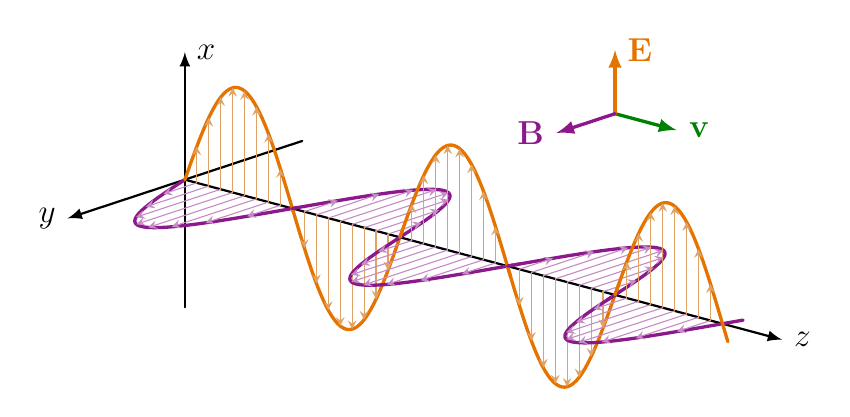
\begin{tikzpicture}[x=(-15:0.9), y=(90:0.9), z=(-150:1.1),
                    line cap=round, line join=round,
                    axis/.style={black, thick,->},
                    vector/.style={>=stealth,->}]
  \large
  \def\A{1.5}
  \def\nNodes{5} % use even number
  \def\nVectorsPerNode{8}
  \def\N{\nNodes*40}
  \def\xmax{\nNodes*pi/2*1.01}
  \pgfmathsetmacro\nVectors{(\nVectorsPerNode+1)*\nNodes}
  \def\vE{{\color{Ecol}\mathbf{E}}}
  \def\vB{{\color{Bcol}\mathbf{B}}}
  
  \def\drawENode{ % draw E node and vectors with some offset
    \draw[Ecol,very thick,variable=\t,domain=\iOffset*pi/2:(\iOffset+1)*pi/2*1.01,samples=40]
      plot (\t,{\A*sin(\t*360/pi)},0);
    \foreach \k [evaluate={\t=\k*pi/2/(\nVectorsPerNode+1);
                           \angle=\k*90/(\nVectorsPerNode+1);}]
                in {1,...,\nVectorsPerNode}{
      \draw[vector,EVcol]  (\iOffset*pi/2+\t,0,0) -- ++(0,{\A*sin(2*\angle+\iOffset*180)},0);
    }
  }
  \def\drawBNode{ % draw B node and vectors with some offset
    \draw[Bcol,very thick,variable=\t,domain=\iOffset*pi/2:(\iOffset+1)*pi/2*1.01,samples=40]
      plot (\t,0,{\A*sin(\t*360/pi)});
    \foreach \k [evaluate={\t=\k*pi/2/(\nVectorsPerNode+1);
                           \angle=\k*90/(\nVectorsPerNode+1);}]
                in {1,...,\nVectorsPerNode}{
      \draw[vector,Bcol!50]  (\iOffset*pi/2+\t,0,0) -- ++(0,0,{\A*sin(2*\angle+\iOffset*180)});
    }
  }
  
  % MAIN AXES
  \draw[axis] (0,0,0) -- ++(\xmax*1.1,0,0) node[right] {$z$};
  \draw[axis] (0,-\A*1.2,0) -- (0,\A*1.2,0) node[right] {$x$};
  \draw[axis] (0,0,-\A*1.2) -- (0,0,\A*1.2) node[left] {$y$};
  
  % SMALL AXES
  \def\xOffset{{(\nNodes-2)*pi/2}}
  \def\yOffset{\A*1.1}
  \def\zOffset{\A*1.1}
  \draw[axis,very thick,vcol] (\xOffset,\yOffset,-\zOffset) -- ++(\A*0.6,0,0) node[right,align=center] {$\vb{v}$}; %\\propagation
  \draw[axis,very thick,Ecol]  (\xOffset,\yOffset,-\zOffset) -- ++(0,\A*0.6,0) node[right] {$\vb{E}$};
  \draw[axis,very thick,Bcol]   (\xOffset,\yOffset,-\zOffset) -- ++(0,0,\A*0.6) node[left] {$\vb{B}$};
  
  % draw (anti-)nodes
  \foreach \iNode [evaluate={\iOffset=\iNode-1;}] in {1,...,\nNodes}{
    \ifodd\iNode \drawBNode \drawENode % E overlaps B
    \else        \drawENode \drawBNode % B overlaps E
    \fi
  }

\end{tikzpicture}



% Electromagnetic wave - circular polarization - color
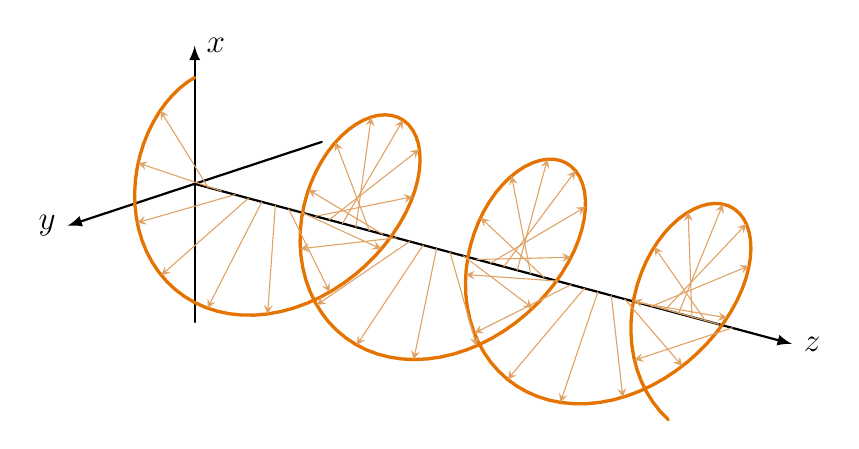
\begin{tikzpicture}[x=(-15:0.9), y=(90:0.9), z=(-150:1.1),
                    line cap=round, line join=round,
                    axis/.style={black, thick,->},
                    vector/.style={>=stealth,->}]
  
  \large
  \def\A{1.5}
  \def\om{1.3}
  \def\nNodes{5} % use even number
  \def\nVectorsPerNode{8}
  \def\N{\nNodes*40}
  \def\xmax{\nNodes*pi/2*1.01}
  \pgfmathsetmacro\nVectors{\nVectorsPerNode*\nNodes}
  \def\vE{\mathbf{E}}
  \def\vB{\mathbf{B}}
  
  % MAIN AXES
  \draw[axis] (0,0,0) -- ++(\xmax*1.1,0,0) node[right] {$z$};
  \draw[axis] (0,-\A*1.3,0) -- (0,\A*1.3,0) node[right] {$x$};
  \draw[axis] (0,0,-\A*1.3) -- (0,0,\A*1.3) node[left] {$y$};
  
  % waves
  \draw[Ecol,very thick,variable=\t,domain=0:\nNodes*pi/2*1.03,samples=\N]
    plot (\t,{\A*cos(\om*\t*360/pi)},{\A*sin(\om*\t*360/pi)});
  
  % draw vectors
  \foreach \k [evaluate={\t=\k*pi/2/\nVectorsPerNode;
                         \angle=\k*90/\nVectorsPerNode;}]
              in {1,...,\nVectors}{
    \draw[EVcol,vector] (\t,0,0) -- ++(0,{\A*cos(\om*2*\angle)},{\A*sin(\om*2*\angle)});
  }
  
\end{tikzpicture}



% Electromagnetic wave SHORT - colored
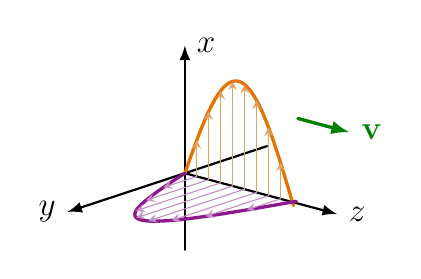
\begin{tikzpicture}[x=(-15:0.9), y=(90:0.9), z=(-150:1.1),
                    line cap=round, line join=round,
                    axis/.style={black, thick,->},
                    vector/.style={>=stealth,->}]
  \large
  \def\A{1.5}
  \def\ymax{1.8}
  \def\nNodes{1} % use even number
  \def\nVectorsPerNode{8}
  \def\N{\nNodes*40}
  \def\xmax{\nNodes*pi/2*1.01}
  \pgfmathsetmacro\nVectors{(\nVectorsPerNode+1)*\nNodes}
  
  % MAIN AXES
  \draw[axis] (0,0,0) -- ++(\xmax*1.4,0,0) node[right] {$z$};
  \draw[axis] (0,-\ymax*0.6,0) -- (0,\ymax,0) node[right] {$x$};
  \draw[axis] (0,0,-\ymax*0.7) -- (0,0,\ymax) node[left] {$y$};
  
  \draw[Ecol,very thick,variable=\t,domain=0:pi/2*1.01,samples=40]
    plot (\t,{\A*sin(\t*360/pi)},0);
  \foreach \k [evaluate={\t=\k*pi/2/(\nVectorsPerNode+1);
                         \angle=\k*90/(\nVectorsPerNode+1);}]
              in {1,...,\nVectorsPerNode}{
    \draw[vector,EVcol]  (\t,0,0) -- ++(0,{\A*sin(2*\angle)},0);
  }
  \draw[Bcol,very thick,variable=\t,domain=0:pi/2*1.01,samples=40]
    plot (\t,0,{\A*sin(\t*360/pi)});
  \foreach \k [evaluate={\t=\k*pi/2/(\nVectorsPerNode+1);
                         \angle=\k*90/(\nVectorsPerNode+1);}]
              in {1,...,\nVectorsPerNode}{
    \draw[vector,Bcol!50]  (\t,0,0) -- ++(0,0,{\A*sin(2*\angle)});
  }
  
  % VECTOR
  \draw[->,very thick,vcol] (\A*1.1,\A*0.8,0) --++ (\A*0.5,0,0) node[right] {$\vb{v}$};
  
\end{tikzpicture}



% Electromagnetic wave SHORT SQUARED - colored
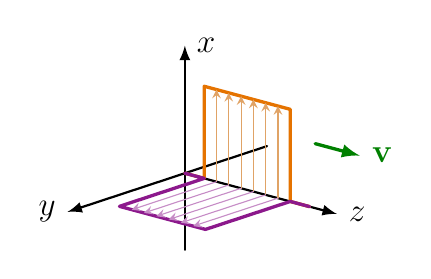
\begin{tikzpicture}[x=(-15:0.9), y=(90:0.9), z=(-150:1.1),
                    line cap=round, line join=round,
                    axis/.style={black, thick,->},
                    vector/.style={>=stealth,->}]
  \large
  \def\A{1.3}
  \def\ymax{1.8}
  \def\nNodes{1} % use even number
  \def\nVectorsPerNode{6}
  \def\N{\nNodes*40}
  \def\xmax{\nNodes*pi/2*1.01}
  \def\wx{\nNodes*pi/2*0.8}
  \def\dx{\nNodes*pi/2*0.18}
  \pgfmathsetmacro\nVectors{(\nVectorsPerNode+1)*\nNodes}
  
  % MAIN AXES
  \draw[axis] (0,0,0) -- ++(\xmax*1.4,0,0) node[right] {$z$};
  \draw[axis] (0,-\ymax*0.6,0) -- (0,\ymax,0) node[right] {$x$};
  \draw[axis] (0,0,-\ymax*0.7) -- (0,0,\ymax) node[left] {$y$};
  
  % IMPULSE
  \draw[Ecol,very thick]
    (0,0,0) --++ (\dx,0,0) --++ (0,\A,0) --++ (\wx,0,0) --++ (0,-\A,0) --++ (\dx,0,0);
  \foreach \k [evaluate={\t=\dx+\k*\wx/(\nVectorsPerNode+1);}] in {1,...,\nVectorsPerNode}{
    \draw[vector,EVcol] (\t,0,0) -- ++(0,\A,0);
  }
  \draw[Bcol,very thick]
    (0,0,0) --++ (\dx,0,0) --++ (0,0,\A) --++ (\wx,0,0) --++ (0,0,-\A) --++ (\dx,0,0);
  \foreach \k [evaluate={\t=\dx+\k*\wx/(\nVectorsPerNode+1);}] in {1,...,\nVectorsPerNode}{
    \draw[vector,Bcol!50] (\t,0,0) -- ++(0,0,\A);
  }
  
  % VECTOR
  \draw[->,very thick,vcol] (\xmax*1.2,\A*0.7,0) --++ (\A*0.5,0,0) node[right] {$\vb{v}$};
  
\end{tikzpicture}



% Electromagnetic wave - black
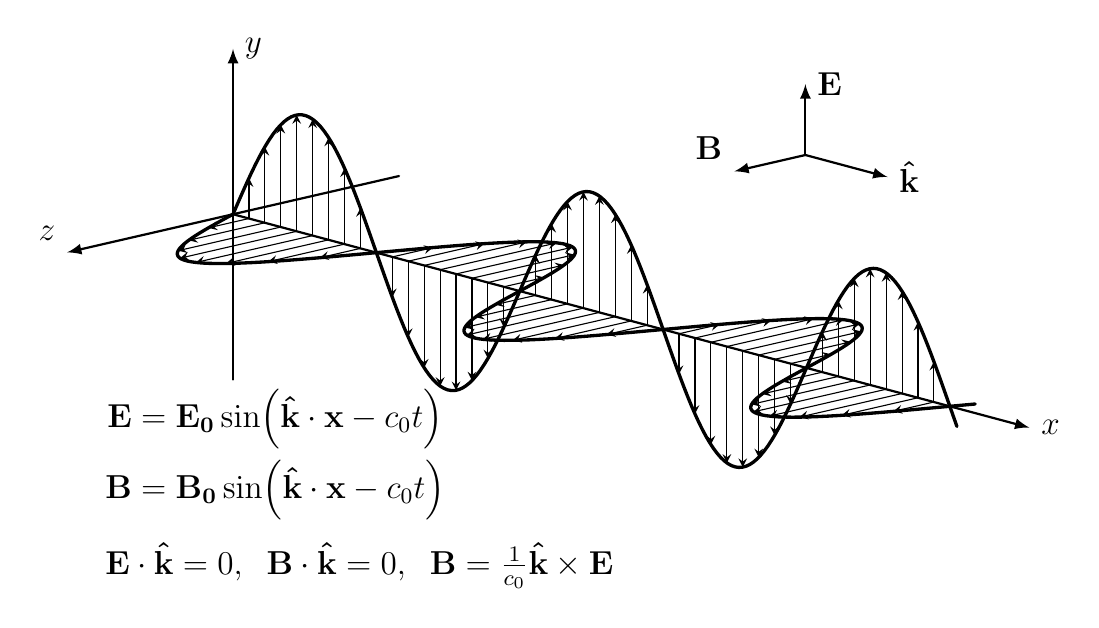
\begin{tikzpicture}[x=(-15:1.2), y=(90:1.0), z=(-150:1.0),
                    line cap=round, line join=round,
                    axis/.style={black, thick,->},
                    vector/.style={>=stealth,->}]
  \large
  \def\A{1.5}
  \def\nNodes{5} % use even number
  \def\nVectorsPerNode{8}
  \def\N{\nNodes*40}
  \def\xmax{\nNodes*pi/2*1.01}
  \pgfmathsetmacro\nVectors{(\nVectorsPerNode+1)*\nNodes}
  
  \def\vE{\mathbf{E}}
  \def\vB{\mathbf{B}}
  \def\vk{\mathbf{\hat{k}}}
  
  % MAIN AXES
  \draw[axis] (0,0,0) -- ++(\xmax*1.1,0,0) node[right] {$x$};
  \draw[axis] (0,-\A*1.4,0) -- (0,\A*1.4,0) node[right] {$y$};
  \draw[axis] (0,0,-\A*1.4) -- (0,0,\A*1.4) node[above left] {$z$};
  
  % SMALL AXES
  \def\xOffset{{(\nNodes-2)*pi/2}}
  \def\yOffset{\A*1.2}
  \def\zOffset{\A*1.2}
  \draw[axis] (\xOffset,\yOffset,-\zOffset) -- ++(\A*0.6,0,0) node[right] {$\vk$};
  \draw[axis] (\xOffset,\yOffset,-\zOffset) -- ++(0,\A*0.6,0) node[right] {$\vE$};
  \draw[axis] (\xOffset,\yOffset,-\zOffset) -- ++(0,0,\A*0.6) node[above left] {$\vB$};
  
  % equation
  \node[above right] at (\xOffset,-0.5*\yOffset,4*\zOffset)
    {$\begin{aligned}
      \vE &= \mathbf{E_0}\sin(\vk\cdot\mathbf{x}-c_0t)\\
      \vB &= \mathbf{B_0}\sin(\vk\cdot\mathbf{x}-c_0t)\\
      \end{aligned}$};
  \node[below right] at (\xOffset,-0.5*\yOffset,4*\zOffset)
    {$\vE\cdot\vk = 0,\;\; \vB\cdot\vk = 0,\;\; \vB = \frac{1}{c_0}\vk\times\vE$};
  
  % waves
  \draw[very thick,variable=\t,domain=0:\nNodes*pi/2*1.01,samples=\N]
    plot (\t,{\A*sin(\t*360/pi)},0);
  \draw[very thick,variable=\t,domain=0:\nNodes*pi/2*1.01,samples=\N]
    plot (\t,0,{\A*sin(\t*360/pi)});
  
  % draw vectors
  \foreach \k [evaluate={\t=\k*pi/2/(\nVectorsPerNode+1);
                         \angle=\k*90/(\nVectorsPerNode+1);
                         \c=(mod(\angle,90)!=0);}]
              in {1,...,\nVectors}{
    \if\c1
      \draw[vector] (\t,0,0) -- ++(0,{\A*sin(2*\angle)},0);
      \draw[vector] (\t,0,0) -- ++(0,0,{\A*sin(2*\angle)});
    \fi
  }
  
\end{tikzpicture}



% Electromagnetic wave - circular polarization
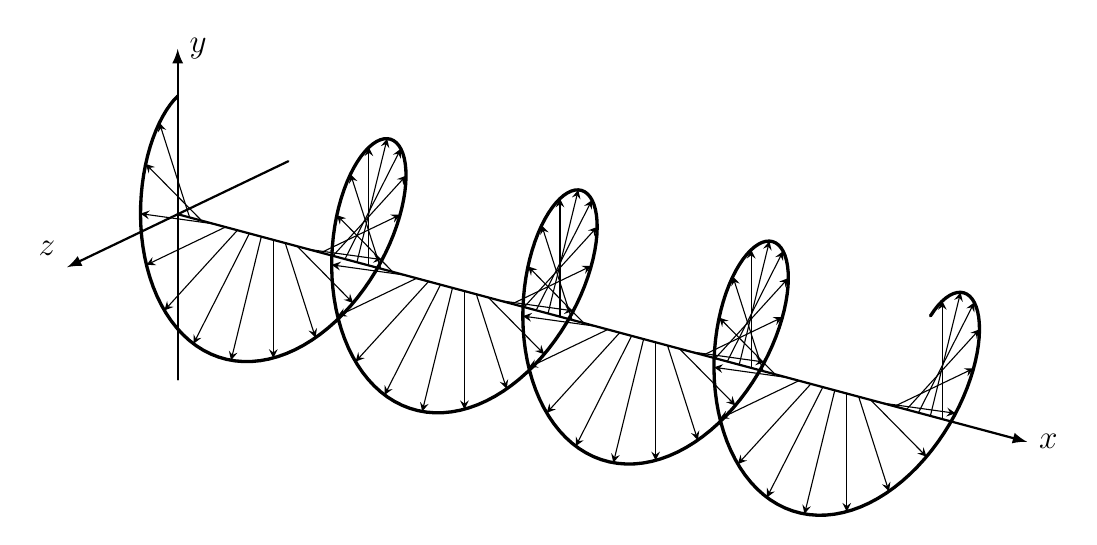
\begin{tikzpicture}[x=(-15:0.8), y=(90:1.0), z=(-150:1.0),
                    line cap=round, line join=round,
                    axis/.style={black, thick,->},
                    vector/.style={>=stealth,->}]
  \large
  \def\A{1.5}
  \def\nNodes{8} % use even number
  \def\nVectorsPerNode{8}
  \def\N{\nNodes*40}
  \def\xmax{\nNodes*pi/2*1.01}
  \pgfmathsetmacro\nVectors{\nVectorsPerNode*\nNodes}
  
  \def\vE{\mathbf{E}}
  \def\vB{\mathbf{B}}
  \def\vk{\mathbf{\hat{k}}}
  
  % MAIN AXES
  \draw[axis] (0,0,0) -- ++(\xmax*1.1,0,0) node[right] {$x$};
  \draw[axis] (0,-\A*1.4,0) -- (0,\A*1.4,0) node[right] {$y$};
  \draw[axis] (0,0,-\A*1.4) -- (0,0,\A*1.4) node[above left] {$z$};
  
  % waves
  \draw[very thick,variable=\t,domain=0:\nNodes*pi/2*1.01,samples=\N]
    plot (\t,{\A*cos(\t*360/pi)},{\A*sin(\t*360/pi)});
  
  % draw vectors
  \foreach \k [evaluate={\t=\k*pi/2/\nVectorsPerNode;
                         \angle=\k*90/\nVectorsPerNode;}]
              in {1,...,\nVectors}{
    \draw[vector] (\t,0,0) -- ++(0,{\A*cos(2*\angle)},{\A*sin(2*\angle)});
  }
  
\end{tikzpicture}



% Electromagnetic wave - colored
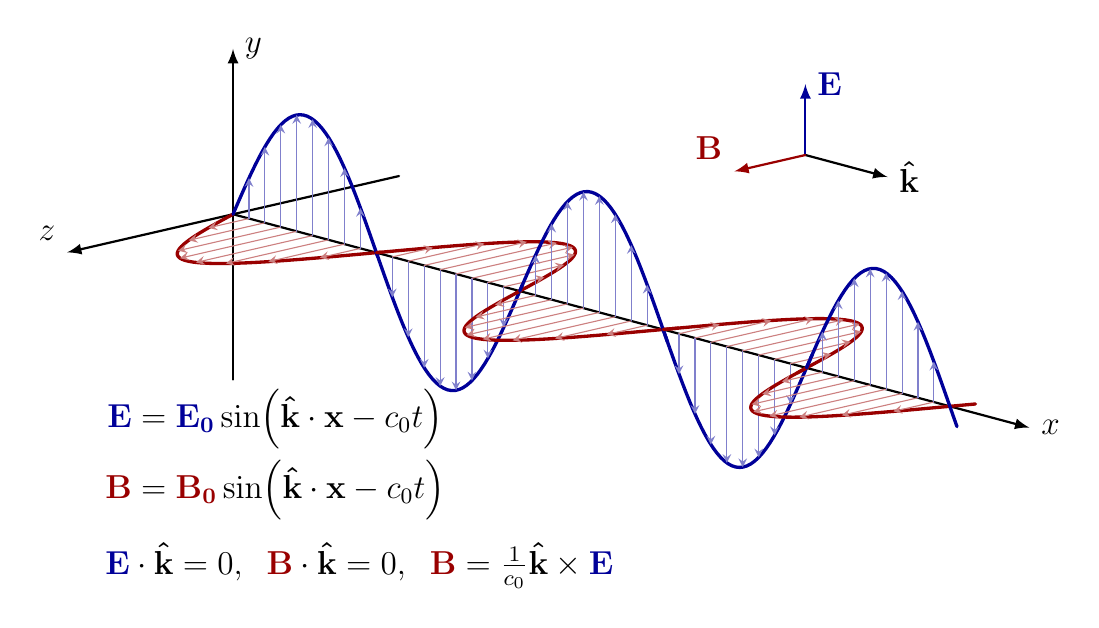
\begin{tikzpicture}[x=(-15:1.2), y=(90:1.0), z=(-150:1.0),
                    line cap=round, line join=round,
                    axis/.style={black, thick,->},
                    vector/.style={>=stealth,->}]
  \large
  \def\A{1.5}
  \def\nNodes{5} % use even number
  \def\nVectorsPerNode{8}
  \def\N{\nNodes*40}
  \def\xmax{\nNodes*pi/2*1.01}
  \pgfmathsetmacro\nVectors{(\nVectorsPerNode+1)*\nNodes}
  
  \def\vE{{\color{myblue}\mathbf{E}}}
  \def\vB{{\color{myred}\mathbf{B}}}
  \def\vk{\mathbf{\hat{k}}}
  
  \def\drawENode{ % draw E node and vectors with some offset
    \draw[myblue,very thick,variable=\t,domain=\iOffset*pi/2:(\iOffset+1)*pi/2*1.01,samples=40]
      plot (\t,{\A*sin(\t*360/pi)},0);
    \foreach \k [evaluate={\t=\k*pi/2/(\nVectorsPerNode+1);
                           \angle=\k*90/(\nVectorsPerNode+1);}]
                in {1,...,\nVectorsPerNode}{
      \draw[vector,myblue!50]  (\iOffset*pi/2+\t,0,0) -- ++(0,{\A*sin(2*\angle+\iOffset*180)},0);
    }
  }
  \def\drawBNode{ % draw B node and vectors with some offset
    \draw[myred,very thick,variable=\t,domain=\iOffset*pi/2:(\iOffset+1)*pi/2*1.01,samples=40]
      plot (\t,0,{\A*sin(\t*360/pi)});
    \foreach \k [evaluate={\t=\k*pi/2/(\nVectorsPerNode+1);
                           \angle=\k*90/(\nVectorsPerNode+1);}]
                in {1,...,\nVectorsPerNode}{
      \draw[vector,myred!50]  (\iOffset*pi/2+\t,0,0) -- ++(0,0,{\A*sin(2*\angle+\iOffset*180)});
    }
  }
  
  % MAIN AXES
  \draw[axis] (0,0,0) -- ++(\xmax*1.1,0,0) node[right] {$x$};
  \draw[axis] (0,-\A*1.4,0) -- (0,\A*1.4,0) node[right] {$y$};
  \draw[axis] (0,0,-\A*1.4) -- (0,0,\A*1.4) node[above left] {$z$};
  
  % SMALL AXES
  \def\xOffset{{(\nNodes-2)*pi/2}}
  \def\yOffset{\A*1.2}
  \def\zOffset{\A*1.2}
  \draw[axis,black] (\xOffset,\yOffset,-\zOffset) -- ++(\A*0.6,0,0) node[right,align=center] {$\mathbf{\hat{k}}$}; %\\propagation
  \draw[axis,myblue]  (\xOffset,\yOffset,-\zOffset) -- ++(0,\A*0.6,0) node[right] {$\mathbf{E}$};
  \draw[axis,myred]   (\xOffset,\yOffset,-\zOffset) -- ++(0,0,\A*0.6) node[above left] {$\mathbf{B}$};
  
  % equation
  \node[above right] at (\xOffset,-0.5*\yOffset,4*\zOffset)
    {$\begin{aligned}
      \vE &= {\color{myblue}\mathbf{E_0}}\sin(\vk\cdot\mathbf{x}-c_0t)\\
      \vB &= {\color{myred} \mathbf{B_0}}\sin(\vk\cdot\mathbf{x}-c_0t)\\
      \end{aligned}$};
  \node[below right] at (\xOffset,-0.5*\yOffset,4*\zOffset)
    {$\vE\cdot\vk = 0,\;\; \vB\cdot\vk = 0,\;\; \vB = \frac{1}{c_0}\vk\times\vE$};
  
  % draw (anti-)nodes
  \foreach \iNode [evaluate={\iOffset=\iNode-1;}] in {1,...,\nNodes}{
    \ifodd\iNode \drawBNode \drawENode % E overlaps B
    \else        \drawENode \drawBNode % B overlaps E
    \fi
  }

\end{tikzpicture}



\end{document}